\documentclass[11pt,reqno,a4paper]{amsart}
%SetFonts

%SetFonts

%%%% Pacotes adicionais para enumeração de items e alinhamento de equações
%%%%
\usepackage{enumitem}
\usepackage{amsmath}
\usepackage{mathtools}


%%%% Escrevendo em português
%%%% 
\usepackage[utf8x]{inputenc}
\usepackage[brazil]{babel}
% \usepackage[latin1]{inputenc} % to offline compiling, use this

%%%% Configurações para output correto de pdf
%%%%
\usepackage[T1]{fontenc}
\usepackage{ae}
\usepackage{aecompl}
\usepackage{amssymb}

%%%% Layout de página
%%%%
\usepackage{fullpage}
\usepackage{setspace}
\usepackage{bbm}

\usepackage{xcolor}
\definecolor{light-gray}{gray}{0.95}
\definecolor{dark-gray}{gray}{0.35}
\newcommand{\code}[1]{\colorbox{light-gray}{\textcolor{dark-gray}{\fontsize{10}{10}{\texttt{#1}}}}}

\begin{document}
\graphicspath{{images/}}
\parindent=0pt

\title{MAC0210 - Laboratório de Métodos Numéricos}
\author{Ygor Sad Machado - N. USP: 8910368}

\pagestyle{plain}
\onehalfspace

\maketitle

\textbf{Relatório}\hfill
\textbf{EP1}\null
\medskip

\noindent\rule{\textwidth}{0.4pt}
\section{Método do ponto fixo}

\medskip
Para compilar e executar a primeira parte do EP, execute \code{make part\_1 \&\& ./part\_1.o}. 

\medskip
O ponto-chave desta primeira parte do EP é encontrar uma função $g(x)$ conveniente. As primeiras tentativas para isso tentaram usar o procedimento mais simples, fazendo $f(x) = 0$ e tentando a partir daí isolar $x$ de maneira tal a encontrar uma função $x = g(x)$. Isso rendeu duas funções:

\begin{align*}
    g_1(x) = \sqrt{\frac{e^x}{2}} &\implies g'_1(x) = \frac{\sqrt{e^x}}{2\sqrt{2}}  \\
    g_2(x) = \ln(2x^2) &\implies g'_2(x) = \frac{2}{x} \\
\end{align*}

\medskip
Nenhuma das duas funções acima é capaz de determinar todas as raízes de $f(x)$, o que não as torna muito práticas. Seria possível, de fato, tentar estimar parte das raízes usando ambas em conjunto, mas isso daria um pouco mais de trabalho.

\medskip
No entanto, com um pouco de destreza é possível construir uma função $g$ intuitiva e que provê todas as raízes. O livro \textit{A First Course in Numerical Computing}, em sua seção \textit{3.4. Newton's method and variants} apresenta um raciocínio interessante, no qual escreve $g$ em função de $f$ e de sua derivada. Vamos usá-lo aqui. Considere então

\begin{equation*}
    g_3(x) = x - \frac{f(x)}{df(x)}
\end{equation*}

\medskip
Se fizermos $g(x) = x$, temos que

\begin{align*}
    x - \frac{f(x)}{df(x)} &= x\\
    \frac{f(x)}{df(x)} &= 0\\
\end{align*}

\medskip
Ora, mas isso só é possível se $f(x) = 0$, já que $df(x)$ não pode ser nula. Vemos então que $g_3(x) = x \implies f(x) = 0$. Assim, definindo de maneira explícita nossa função $g_3$, temos

\begin{equation*}
    g_3(x) = x - \frac{e^x - 2x^2}{e^x - 4x}
\end{equation*}

\medskip
Aplicando tal função ao método do ponto fixo, usando 0, 1 e 3 como ponto de partida, obtemos respectivamente os seguintes valores para as raízes de f:

\bigskip
\begin{itemize}
    \item $x^{*}_1$ = -0.5398352769 $\implies f(x^{*}_1) = 7.73304×10^{-12}$ 
    \item $x^{*}_2$ = 1.4879620655 $\implies f(x^{*}_2) = -2.8 × 10^{-12}$
    \item $x^{*}_3$ = 2.6178666131 $\implies f(x^{*}_3) = 1.074×10^{-10}$ 
\end{itemize}

\bigskip
O interessante de se observar aqui é, para os três cenários, o método converge usando em média 4 iterações. Além disso, executando alguns testes degenerados, é possível notar que, para essa função $f$ em particular, independentemente do número máximo de iterações aceito, o método tolera valores negativos de $x$ absurdamente baixos. Por exemplo:

\bigskip
\begin{itemize}
    \item $x_0 = -100320524.0 \implies x^{*} = -0.5398352769$ com 31 iterações
    \item $x_0 = -55555555555 \implies x^{*} = -0.5398352769$ com 40 iterações
\end{itemize}

\bigskip
No entanto, a depender do número de máximo de iterações permitido, ele pode falhar para $x$ positivos relativamente pequenos. Por exemplo, fixando o máximo de 100 iterações, o método diverge já com $x_0 = 99$. Contudo, se formos um pouco mais permissivos e aceitarmos 1000 iterações:

\bigskip
\begin{itemize}
    \item $x_0 = 99$ converge após 103 iterações
    \item $x_0 = 467$ converge após 471 iterações
\end{itemize}

\bigskip
Isso, naturalmente, é resultado tanto da componente exponencial de $f$, que gera valores demasiado altos quanto da permissividade dos parâmetros usados no método.

\medskip
Um outro detalhe relevante acerca desta implementação é a \code{struct iteration\_result}. Ela serve como encapsuladora dos resultados de uma execução do método do ponto fixo, permitindo que o cliente da função \code{fixed\_point\_method} saiba quando se a execução divergiu, o número de iterações transcorridas, e o último valor calculado para $x_k$ – no código armazenado na variável \code{root}.

\medskip
Por fim, convém notar que foi adotado como critério de parada $|f(x)| \leq \text{tol}$. Esse critério não apenas é mais intuitivo, como permite que $f$ apresente desníveis próximos às raízes sem que isso afete o resultado do método.

\bigskip
\noindent\rule{\textwidth}{0.4pt}
\section{Bacias de Newton}

\medskip
Para compilar e executar a segunda parte do EP, rode \code{make part\_2 \&\& ./part\_2.o}. Para gerar o gráfico associado, execute \code{gnuplot plot.gp -p}.

\medskip
Para a segunda parte do EP, o algoritmo que busca as bacias de Newton foi executado para algumas funções a fim de experimentação, sendo as cinco abaixo as escolhidas para constar nesse relatório:

\begin{align}
    f_1(x) &= x^3 - 3x + 1 \\
    f_2(x) &= 2 * cosh(x / 4) - x \\
    f_3(x) &= x^5 - 1 \\
    f_4(x) &= 2x^4 - x^3 + 5x \\
    f_5(x) &= x^7 - 1
\end{align}

\bigskip
Essas funções foram escolhidas pelos resultados gráficos interessantes e por terem apresentado alguns comportamentos recorrentes em outras funções semelhantes. Ao final deste relatório estão presentes as imagens geradas a partir dessas funções.

\medskip
Um ponto curioso a se observar é a presença constante de simetria em todas as imagens geradas. Mesmo a função $f_2$, que faz uso da função $cosh$ apresenta um padrão de simetria – bastante complexo, note-se.

\medskip
Outro fator relevante a ser mencionado é a forma com que funções semelhantes geram padrões semelhantes. $f_3$, por exemplo, possui bacias com formato semelhante à função $f_5$, apresentada no enunciado deste EP. A única diferença entre elas é o número de eixos radiais: enquanto a função $f_3$ possui cinco eixos, por ser de grau 5, a função $f_7$ possui sete deles, uma vez que é de grau 7.

\medskip
Acerca da implementação desta parte do EP, novamente foi escolhido como critério de parada $|f(x)| \leq \text{tol}$. Além de intuitivo, ele não apresenta dependência nos valores de $x$, permitindo que desníveis abruptos próximos às raízes não interfiram na precisão do método.

\medskip
É relevante, também, ressaltar o limite de iterações conservador adotado – 100 iterações. Tal limite foi determinado por pura questão de segurança, para o caso de haver algum caso degenerado na qual o método convirja após um número anormalmente alto de iterações. No entanto, a observação prática mostrou que, na maior parte das vezes, era possível determinar que o método não iria convergir com muito menos iterações - 40 execuções parece ser um valor factível para isso, nas funções estudada.

\medskip
Por fim é conveniente mencionar alguns detalhes do \textit{modus operandi} da função \code{output\_for}, responsável por gerar a saída associada a cada valor retornado pela função \code{newton}. Seu funcionamento é baseado na associação a um número sequencial, a partir de 1, a cada valor possível de ser gerado por \code{newton}. O intuito disso é tornar mais fácil a geração do gráfico final, já que não será necessário lidar com números complexos ou racionais, apenas inteiros pequenos. No entanto, para que isso seja possível, é necessário conhecer de antemão as raízes de cada função $f$, o que pode ser feito executando o método \code{newton} para diversos valores de $x$ até que se tenham boas estimativas para as raízes.

\medskip
Outro ponto negativo de \code{output\_for} é que ela sempre precisa gerar números a partir de 1, já que o script responsável pela plotagem utiliza comandos do gnuplot que não conseguem receber 0 como entrada. Isso é inconveniente, pois implica que os \textit{arrays} auxiliares utilizados não podem ter o índice 0 preenchido com um valor válido. No entanto, não chega a ser algo que causa grandes anomalias ao processo do EP como um todo.

\begin{figure}[p]
    \centering
    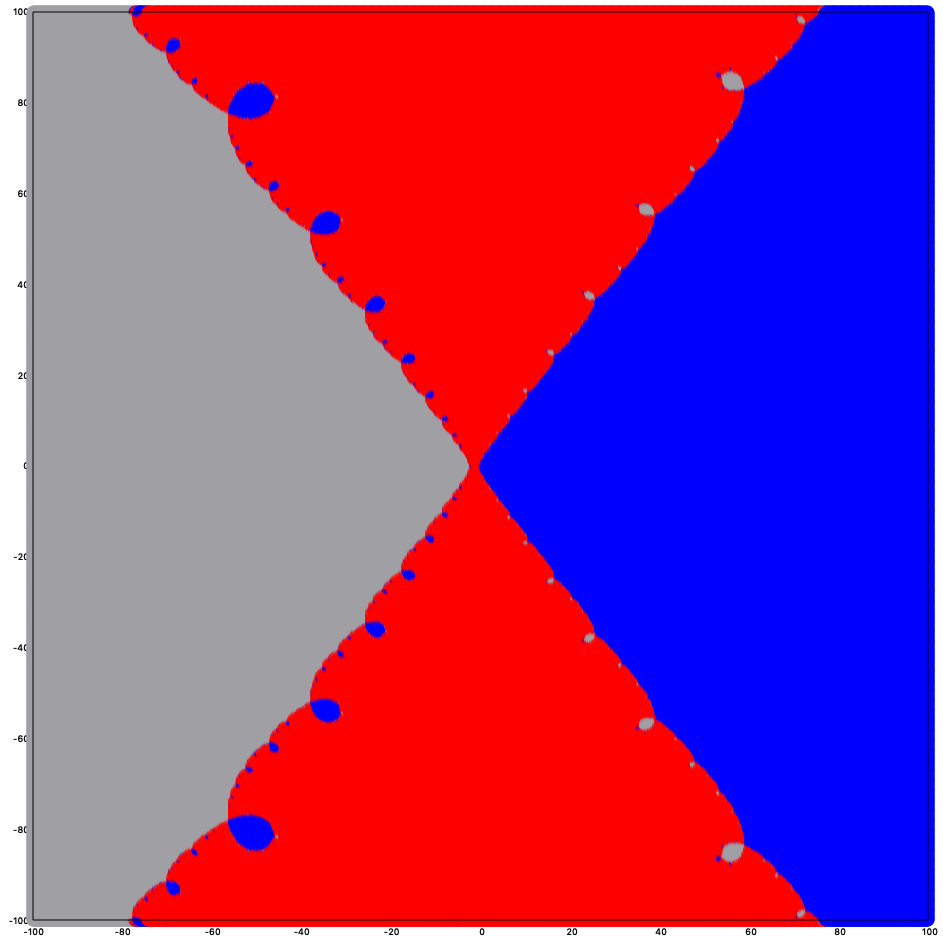
\includegraphics[width=15cm]{function_1.png}
    \caption{Bacias geradas pela função $x^3 - 3x + 1$ a partir dos argumentos $l = -10$, $u = 10$ e $p = 700$.}
    \label{fig:images/function_1}
\end{figure}

\begin{figure}[p]
    \centering
    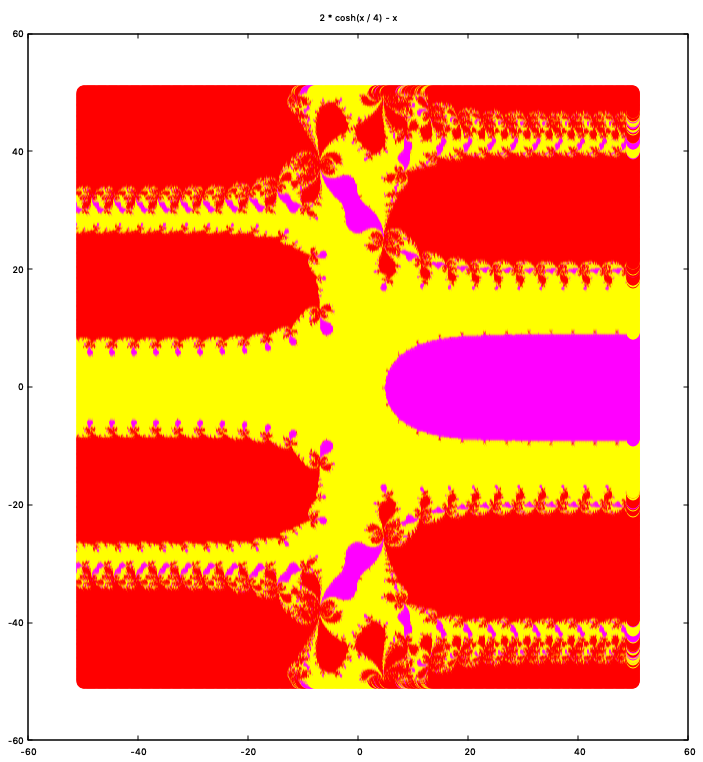
\includegraphics[width=15cm]{function_2.png}
    \caption{Bacias geradas pela função $2cosh(\frac{x}{4}) - x$ a partir dos argumentos $l = -50$, $u = 50$ e $p = 800$.}
    \label{fig:function_2}
\end{figure}

\begin{figure}[p]
    \centering
    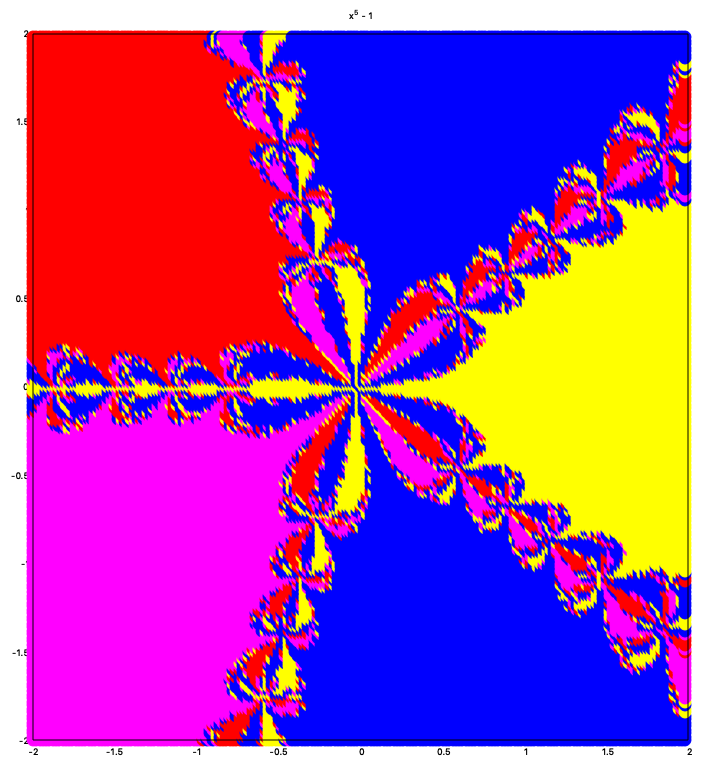
\includegraphics[width=15cm]{function_3.png}
    \caption{Bacias geradas pela função $x^5 - 1$ a partir dos argumentos $l = -2$, $u = 2$ e $p = 200$.}
    \label{fig:function_3}
\end{figure}

\begin{figure}[p]
    \centering
    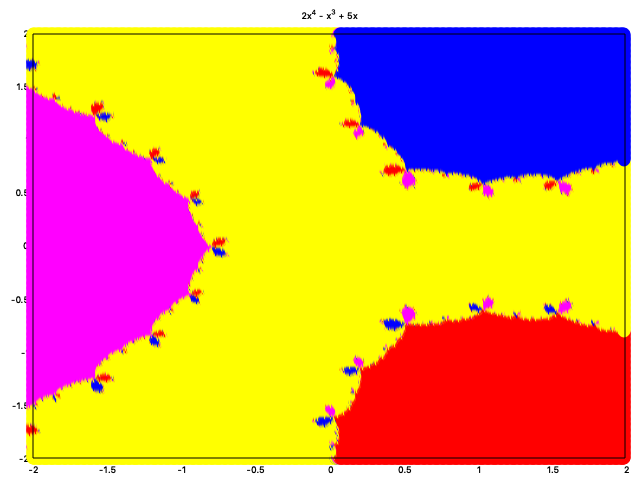
\includegraphics[width=15cm]{function_4.png}
    \caption{Bacias geradas pela função $2x^4 - x^3 + 5x$ a partir dos argumentos $l = -2$, $u = 2$ e $p = 500$.}
    \label{fig:function_4}
\end{figure}

\begin{figure}[p]
    \centering
    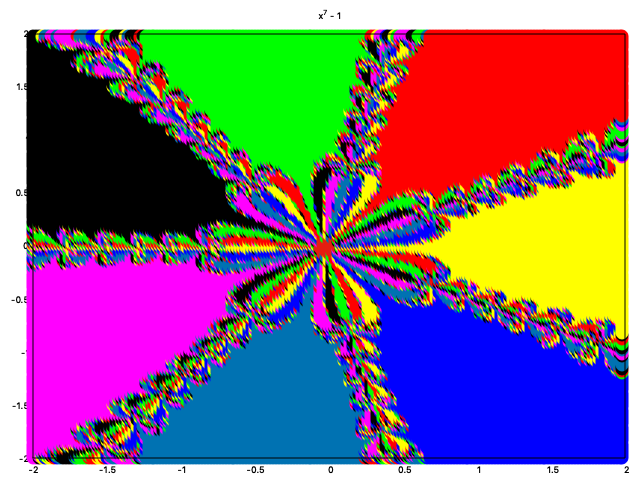
\includegraphics[width=15cm]{function_5.png}
    \caption{Bacias geradas pela função $x^7 - 1$ a partir dos argumentos $l = -2$, $u = 2$ e $p = 200$.}
    \label{fig:function_5}
\end{figure}

\begin{figure}[p]
    \centering
    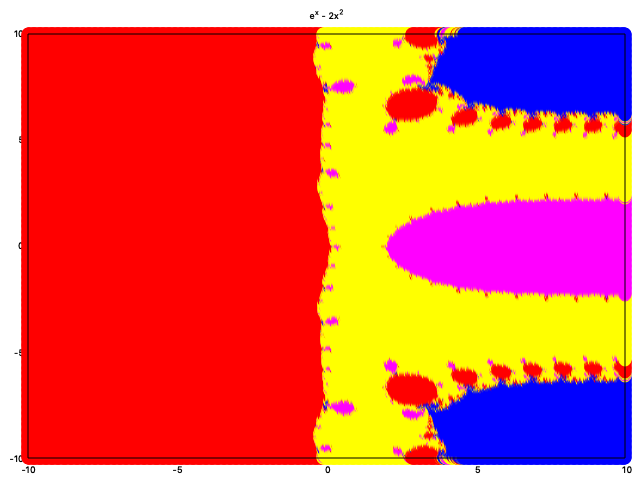
\includegraphics[width=15cm]{function_6.png}
    \caption{Bacias geradas pela função $e^x - 2x^2$ a partir dos argumentos $l = -2$, $u = 2$ e $p = 200$.}
    \label{fig:function6}
\end{figure}


\endgroup
\end{document}